\documentclass[a4paper,oneside,12pt]{article}
\usepackage[margin=0.7in]{geometry}
\usepackage{tikz}
\usepackage[cm-default]{fontspec}
\usepackage{xunicode}
\usepackage{xltxtra}
\usepackage{amsfonts}
\usepackage{amssymb}
\usepackage{amsmath}
\usepackage[utf8]{inputenc}
\usepackage[greek]{babel}
\usepackage{xgreek}
\usepackage{algpseudocode, listings}
\setmainfont[Mapping=tex-text]{CMU Serif}
\usepackage{titling}
\newcommand{\N}{\ensuremath{\mathbb N} }
\newcommand{\Z}{\ensuremath{\mathbb Z} }
\newcommand{\A}{\ensuremath{\mathcal A} }
\newcommand{\pset}[1]{\ensuremath{\mathcal P( #1 )}}
\newcommand{\pr}[1]{\ensuremath{\mathbb P [ #1 ]}}
\renewcommand{\vec}[1]{\ensuremath{\mathbf {  #1 }}}
\newcommand{\ev}[1]{\ensuremath{\mathbb E [ #1 ]}}
\newcommand{\R}{\ensuremath{\mathbb R}}
\DeclareMathOperator{\Ima}{Im}
\usepackage{float}

\newcommand*{\QEDA}{\hfill\ensuremath{\blacksquare}}
\newcommand*{\QEDB}{\hfill\ensuremath{\square}}
\usepackage[usenames,dvipsnames]{pstricks}
\usepackage{epsfig}
\usepackage{pst-grad} % For gradients
\usepackage{pst-plot}
\setlength{\droptitle}{-5em}
\usepackage{graphicx}

\makeatletter
\def\maxwidth{%
  \ifdim\Gin@nat@width>\linewidth
    \linewidth
  \else
    \Gin@nat@width
  \fi
}
\makeatother

\title{ \textbf{Νευρο-Ασαφής Έλεγχος \& Εφαρμογές}  \\ Εργαστηριακή Άσκηση \\ Q Learning}
\author{Όνομα: Μάριος Παπαχρήστου \\ Αριθμός Μητρώου: 03115101 Σχολή ΗΜΜΥ \\ e-mail: \texttt{papachristoumarios@gmail.com}  \\ \line(1,0){500}}
\date{\emph{“Incorporating general intelligence, bodily intelligence, emotional intelligence, spiritual intelligence, political intelligence and social intelligence in AI systems are part of the future deep learning research. ” -- Amit Ray, Compassionate Artificial Intelligence}} 
\lstset{basicstyle=\ttfamily,breaklines=true}

\begin{document}

\maketitle

\section{Σκοπός Εργασίας}

Σκοπός της παρούσας εργασίας είναι η ανάπτυξη ενός ελεγκτή state-feedback διακριτού χρόνου για τη σταθεροποίηση ενός ΓXA συστήματος με χρήση Q Learning βάσει τετραγωγνικού κριτηρίου κόστους. Συγκεκριμένα δίνεται το σύστημα 

$$x_{k+1} = A x_k + B u_k$$

με δυναμικούς πίνακες 

\begin{equation} \label{eq1}
A = \begin{pmatrix} 
	0 & 1 & 0 \\
	0 & 0 & 1 \\
	0 & 0 & 0
\end{pmatrix} \qquad
B = \begin{pmatrix}
	0 \\ 0 \\ 1 
\end{pmatrix}
\end{equation} 

Και το τετραγωνικό κριτήριο κόστους άπειρου ορίζοντα 

$$J = \sum_{i = 0}^\infty (x_i^T x_i + \rho u[i]^2) \qquad \rho > 0$$


\section{Q-Learning}

Θέλουμε να βρούμε βέλτιστο ελεγκτή $u^*_k = - K x_k$ τέτοιο ώστε το σύστημα να είναι ασυμπτωτικά ευσταθές και να ελαχιστοποιείται το κριτήριο κόστους $J$. Με χρήση ενισχυτικής μάθησης, και συγκεκριμένα Q-Learning, μπορούμε να βρούμε αυτή την είσοδο, αγνοώντας τη δυναμική του συστήματος. Θέλουμε να λύσουμε το εξής πρόβλημα βελτιστοποίησης

$$\min_{u_1, \dots, u_T} \sum_{k = 1}^T r_k(x_k, u_k)$$
$$\mathrm{s.t.}\; x_{k+1} = f(x_k, u_k)$$

Στην περίπτωση μας η συνάρτηση $r_k(x_k, u_k)$ είναι η $r_k(u_k, x_k) = x_k^Tx_k + \rho u_k^2$. Εισάγουμε την Q-function για την αξιολόγηση μιας πολιτικής $K$ ως την cost το go συνάρτηση 

\begin{equation}
Q_K(x_k, u_k) \sum_{t \ge k} r_t(x_t, u_t) = r_k(x_k, u_k) + Q_K(x_{k+1}, u_{k+1}) = r_k(x_k, u_k) + x_{k+1}^TP_Kx_{k+1}
\end{equation}

όπου ο όρος $x_{k+1}^T P_K x_{k+1}$ είναι το cost-to-go. Η παραπάνω σχέση μπορεί να λυθεί με δυναμικό προγραμματισμό προκειμένου να λάβουμε την βέλτιση συνάρτηση $Q^*_K(x_k, u_k)$ από την εξίσωση του Bellman

$$Q_K^*(x_k, u_k) = r_k(x_k, u_k) + Q^*_K(x_{k+1}, u_{k+1})$$

Για την ανεύρεση του βέλτιστου κόστους $J^* = x_0^TP^*x_0$ για το πρόβλημα. Η συνάρτηση ποιότητας μπορεί να γραφεί ως

$$Q_K(x_k, u_k) = z_k^T\begin{pmatrix}
	I + A^TPA & B^T P A \\
	A^TPB & \rho + B^T P B 
\end{pmatrix}z_k = z_k^T H z_k$$

όπου $z_k = \begin{pmatrix} x_k \\ u_k \end{pmatrix}$ το επαυξημένο διάνυσμα. Παρατηρούμε ότι ορίζοντας το διάνυσμα $\bar z_k = \mathrm {vec} (z_k z_k^T)$ και το διάνυσμα $\bar H = \mathrm{vec} (H)$ η εξίσωση (2) γράφεται

$$\bar H^T (\bar z_k - z_{k+1}) = r_k$$

Για την εύρεση της $H$ θεωρούμε τους πίνακες 

$$R = (r_1, \dots, r_T)^T \qquad 
Z = \begin{pmatrix}
	[\bar z_0 - \bar z_1]^T \\
	\vdots \\
	[\bar z_{T-1} - \bar z_T]^T
\end{pmatrix}$$ 

Και η παραπάνω εξίσωση λαμβάνει τη μορφή γραμμικού συστήματος

$$Z \bar H = R$$

η οποία έχει λύση την $\bar H = Z^+ R$. Στη συνέχεια επαναφέρουμε τον πίνακα στην αρχική του μορφή 

$$H = \begin{pmatrix}
	H_{xx} & H_{xu} \\
	H_{ux} & H_{uu}
\end{pmatrix} \qquad \text{όπου } H = H^T > 0$$

Ο βέλτιστος νόμος ελέγχου βρίσκεται με το ακρότατο ως προς $u_k$ της συνάρτησης ποιότητας 

$$\frac{\partial Q_K(x_k, u_k)} {\partial u_k} = 0 \iff K^* = H_{uu}^{-1} H_{ux}$$

Για τη συλλογή των δειγμάτων χρησιμοποιείται μια τυχαία είσοδος $u_k = - L x_k, \; L \sim \mathcal N(0, 1_{3 \times 1})$.

Στην υλοποίησή μας με MATLAB, η υλοποίηση της παραπάνω διαδικασίας γίνεται με τη χρήση της ακόλουθης συνάρτησης

\lstinputlisting[language=MATLAB]{q_learning.m}


\section{Ιδανική Περίπτωση} 

Η εύρεση ελεκγτή $u_k = K \vec x_k$ ισοδυναμεί με την επίλυση της Αλγεβρικής Εξίσωσης Ricatti για συστήματα διακριτού χρόνου

$$A^T P A - A^T P B (B^T P B + R)^{-1} B^T P A = -Q$$

όπου $Q = I \ge 0, R = \rho > 0$ για την ανεύρεση της βέλτιστης εισόδου 

$$u^*_k = - (R + B^TPB)^{-1})B^T P A x_k$$

Με χρήση του MATLAB επιλύουμε τη Ricatti και λαμβάνουμε τις τιμές

\begin{lstlisting}
Kid =

   1.0e-16 *

         0   -0.2184    0.7943

>> Pid

Pid =

    1.0000    0.0000   -0.0000
    0.0000    2.0000    0.0000
   -0.0000    0.0000    3.0000

\end{lstlisting}

\newpage
\section{Σύγκριση Αποτελεσμάτων}

Θεωρήσαμε αρχική συνθήκη $x_0 = (0.1, 0.1)^T$. Για το ιδανικό σύστημα έχουμε τις εξής αποκρίσεις για το διάνυσμα κατάστασης και την είσοδο

\begin{figure}[H]
\centering
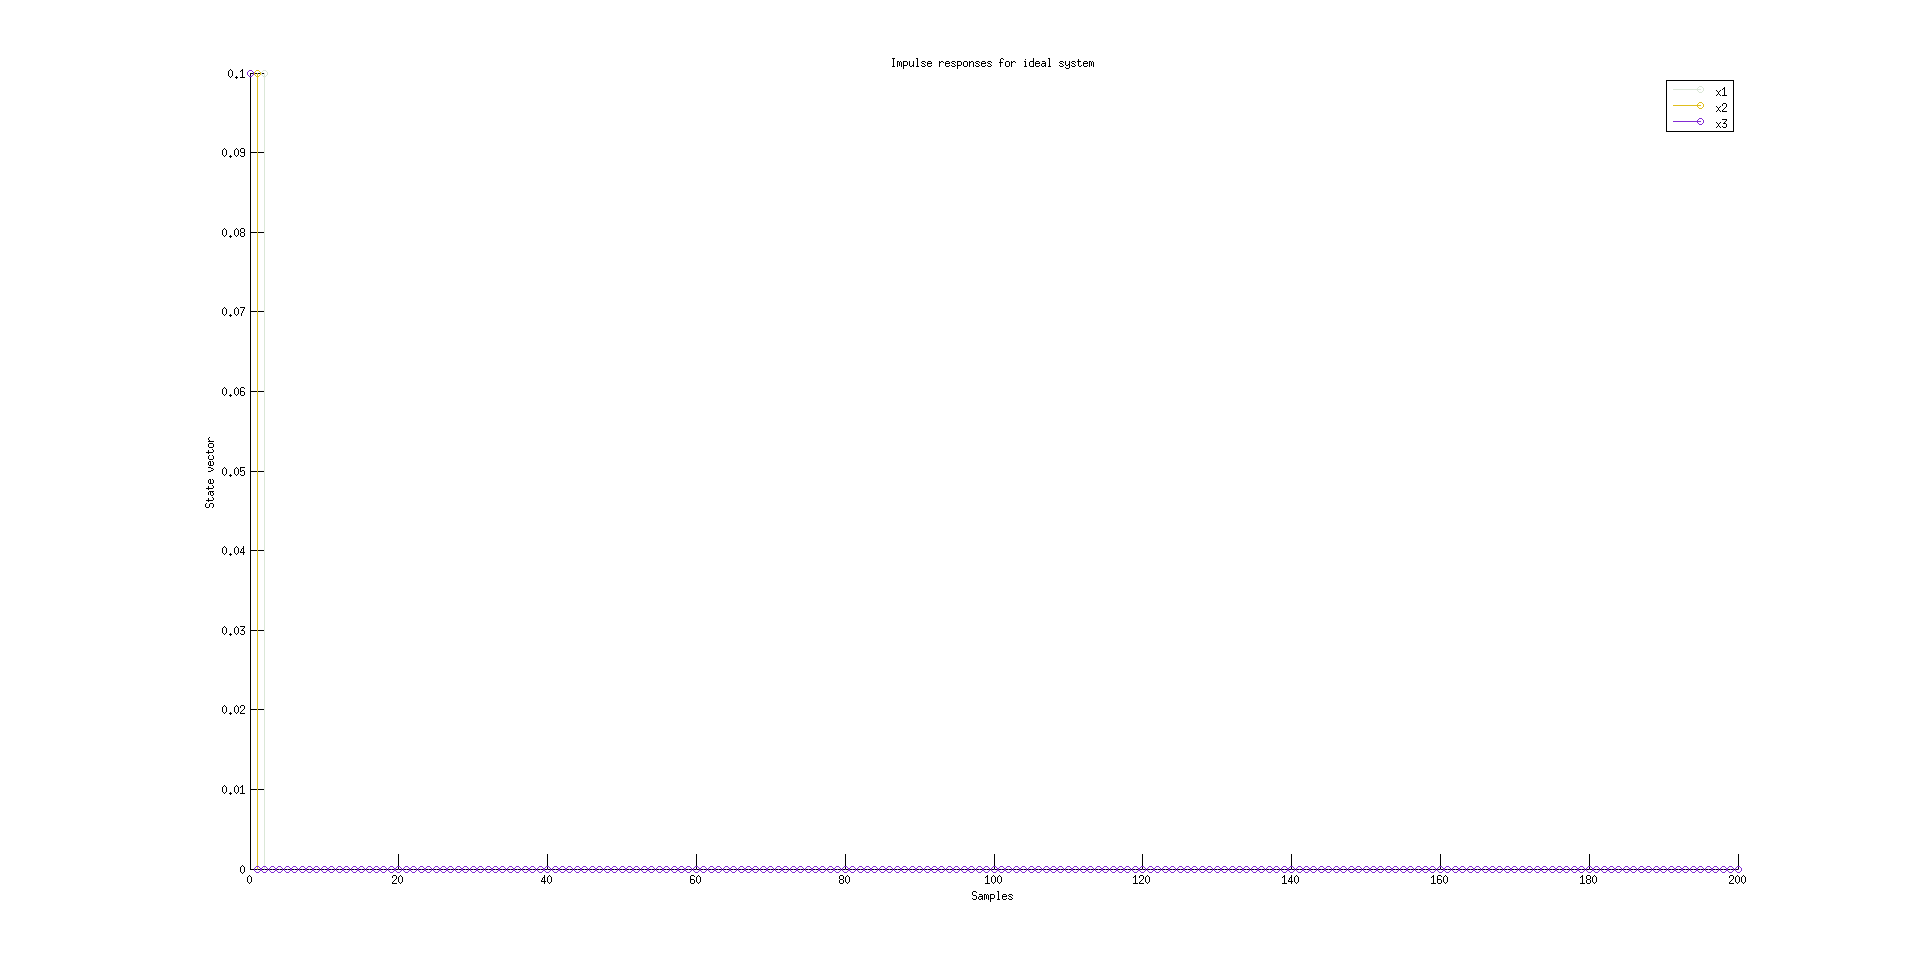
\includegraphics[scale=0.35]{ideal_state.png} \\
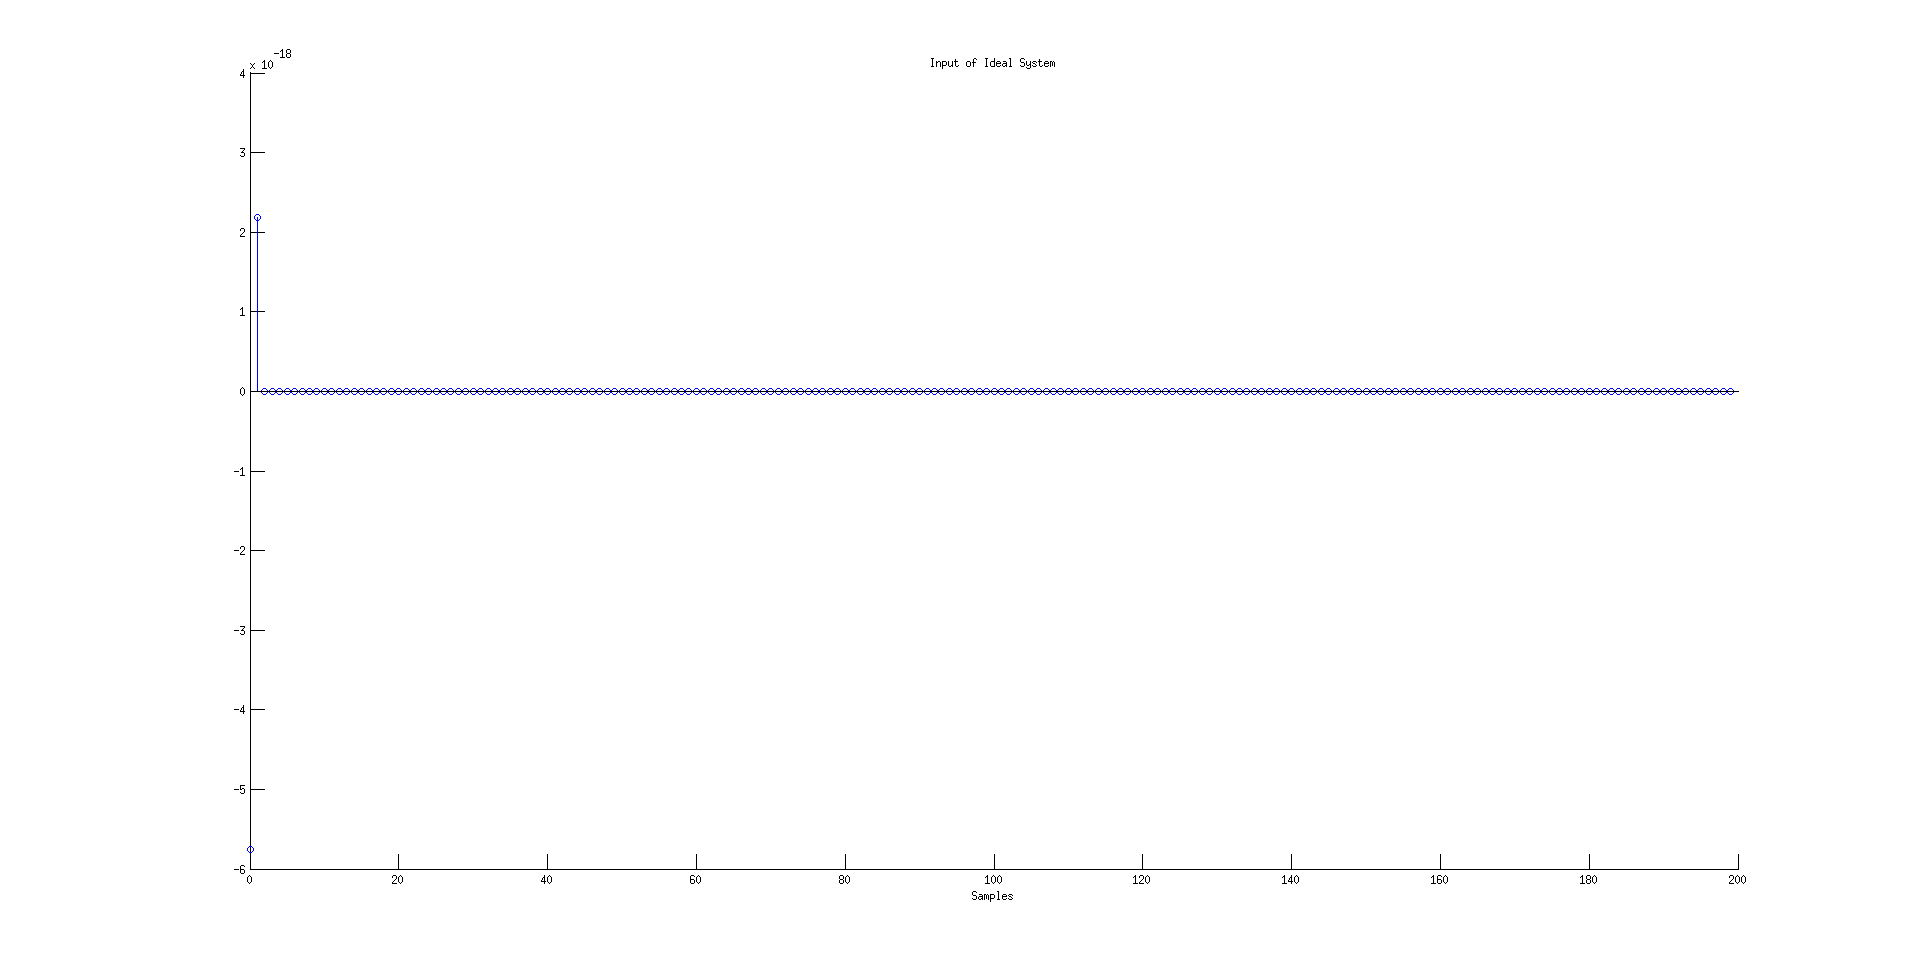
\includegraphics[scale=0.35]{ideal_input.png}
\caption{Ιδανικό Σύστημα (αναλυτική λύση της Ricatti)}
\label{}
\end{figure}


Για το σύστημα που σχεδιάσαμε με Q-Learning

\begin{figure}[H]
\centering
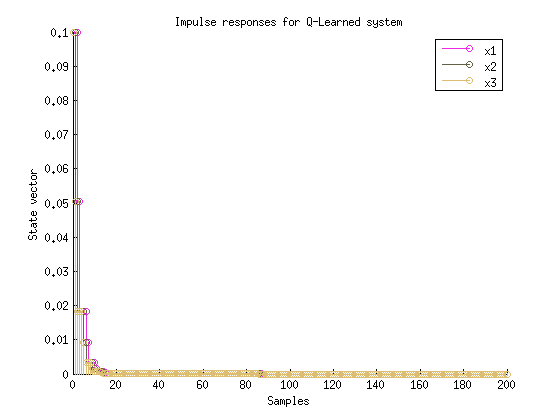
\includegraphics[scale=1.0]{q_state.png} \\
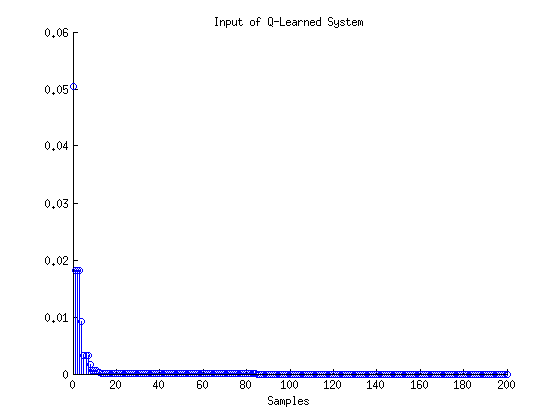
\includegraphics[scale=1.0]{q_input.png}
\caption{Σύστημα με Q-Learning $K = (-0.2781,    0.4261,   -0.6527)$ }
\label{}
\end{figure}

Για τη χρήση τυχαίων εισόδων
\begin{figure}[H]
\centering
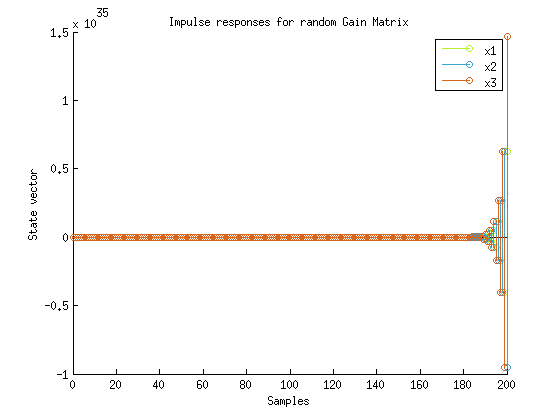
\includegraphics[scale=1.0]{random_state.png} \\
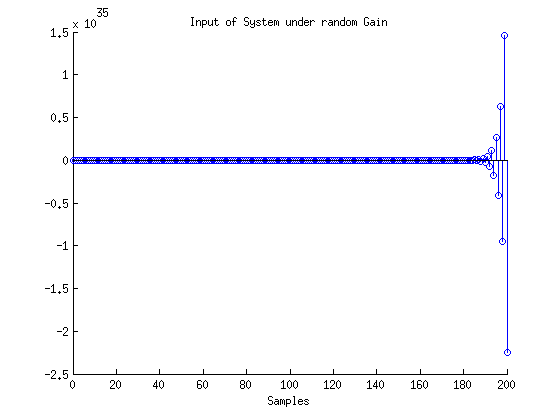
\includegraphics[scale=1.0]{random_input.png}
\caption{Δείγματα με τυχαία είσοδο $L = (1.2178,   -1.4951,    0.0373)$}
\label{}
\end{figure}

Παρατηρούμε ότι το σύστημα από το οποίο πήραμε τα δείγματα είχε ασταθή συμπεριφορά, παρόλα αυτά μάθαμε μια τιμή gain η οποία έκανε το σύστημά μας ευσταθές. 

\section{Πηγαίος Κώδικας}

Το κύριο αρχείο \texttt{main.m}

\lstinputlisting[language=matlab]{main.m}

Για τον υπολογισμό των $H, K$

\lstinputlisting[language=matlab]{q_learning.m}

Για τον υπολογισμό των $\bar z_k$

\lstinputlisting[language=matlab]{quad_comb.m}


\begin{thebibliography}{9}

\bibitem{paper} Bradtke, Steven J. "Reinforcement learning applied to linear quadratic regulation." Advances in neural information processing systems. 1993.

\end{thebibliography}

\end{document}




